\documentclass[class=jsarticle, crop=false, dvipdfmx, fleqn]{standalone}
%% preamble for Numerical-structure-analysis report

\input{/Users/User/Documents/Project/TeX/preamble/mypreamble}

%% titles
\title{先端データ解析論 レポート}
\author{37-196360 \quad 森田涼介}


%% setting for listings
\newtcbinputlisting[auto counter]{\reportlisting}[3][]{%
	listing file = {#3},
	listing options = {language=python, style=tcblatex, numbers=left, numberstyle=\tiny},
	listing only,
	breakable,
	toprule at break = 0mm,
	bottomrule at break = 0mm,
	left = 6mm,
	sharp corners,
	drop shadow,
	title = Listings \thetcbcounter : \texttt{#2},
	label = #1,
	}



%% title format
\usepackage{titlesec}
\titleformat{\section}{\LARGE}{宿題\thesection}{0zw}{}
\newcommand{\sectionbreak}{\clearpage}
\titleformat{\subsection}{\Large}{\Alph{subsection})}{0zw}{}

\begin{document}
\section{}

二乗ヒンジ損失に基づく適応正則化分類を,
線形モデル
\begin{equation}
    f_{\bm{\theta}} (\bm{x}) = \qty(x^{(1)}\ x^{(2)}\ 1) \bm{\theta}
\end{equation}
に対して実装する。

損失は
\begin{align}
    J(\bm{\mu},\ \bm{\Sigma})
        & = \qty(\max(0,\ 1 - \bm{\mu}^\mathrm{T} \phi(\bm{x}) y))^2
            + \phi(\bm{x})^\mathrm{T} \bm{\Sigma} \phi(\bm{x})
            \notag \\
        & \ \qquad
            + \gamma \qty{
            \log\frac{\det(\tilde{\bm{\Sigma}})}{\det{\bm{\Sigma}}}
            + \mathrm{tr}\qty(\tilde{\bm{\Sigma}}^{-1} \bm{\Sigma})
            + (\bm{\mu} - \tilde{\bm{\mu}})^\mathrm{T} \tilde{\bm{\Sigma}}^{-1} (\bm{\mu} - \tilde{\bm{\mu}})
            - d
            }
    \label{eq:loss}
\end{align}
と表され,パラメータの更新式は次のように表される。
\begin{align}
    & \bm{\mu} \leftarrow \bm{\mu} + \frac{y \max(0,\ 1 - \bm{\mu}^\mathrm{T} \phi(\bm{x}) y)}{\phi(\bm{x})^\mathrm{T} \bm{\Sigma} \phi(\bm{x}) + \gamma} \bm{\Sigma} \phi(\bm{x}) \\
    & \bm{\Sigma} \leftarrow \bm{\Sigma} - \frac{\bm{\Sigma} \phi(\bm{x}) \phi(\bm{x})^\mathrm{T} \bm{\Sigma}}{\phi(\bm{x})^\mathrm{T} \bm{\Sigma} \phi(\bm{x}) + \gamma}
\end{align}

\(\gamma = 1.0\),ミニバッチのサイズを10とし,全データに対し50回イタレーションを回したときの結果を,
以下の図\ref{fig:result}に示す。
これを見ると,異常値に対してロバストな解が得られていることがわかる。
プログラムは\pageref{listing:assignment2}ページのListing \ref{listing:assignment2}に示した。

\begin{figure}[H]
    \centering
    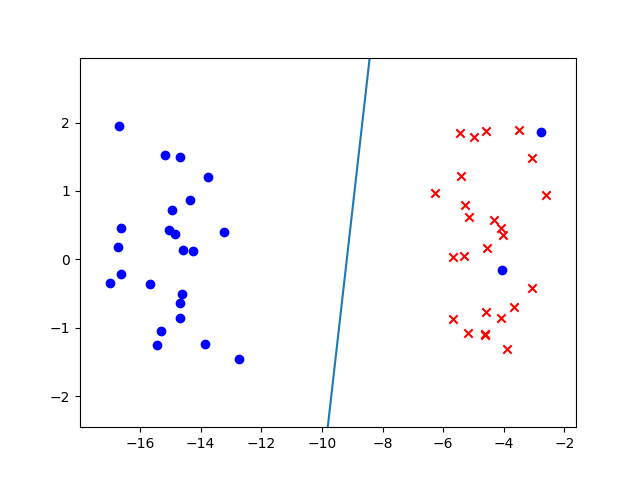
\includegraphics[clip, width=12cm]{../figures/assignment2_result}
    \caption{結果}
    \label{fig:result}
\end{figure}


\end{document}
